\section{Dependency Graph}
A Dependency Graph is a graphical representation of the which module is dependent on which other modules. A Dependency Graph is often used as a preliminary step to creating an overview of the system. Dependency Graph also gives overveiw of how good is the design of the system.
OpenSCAD being were huge software it would be difficult to make the dependency graph of whole software. So, here are some of Dependency Graph of OpenSCAD is as following-:
\begin{enumerate}
	\item \textbf{Dependency graph of Geometery Evaluator:} Figure \ref{fig:geometryevaluator8hdepincl} shows the modules on which the comment.h module is dependent.
	\item \textbf{Caller graph of Geometery Evaluator:} Figure \ref{fig:geometryevaluator8hincl} shows the modules that use the module comment.h.
	\item \textbf{Caller graph of progress.h:} Figure \ref{fig:progress8hdepincl} show the modules that uses the module ParameterWidget.h.
	\item \textbf{Caller graph of find\_root\_tag:} Figure \ref{fig:findRootTag} show the functions that uses find\_root\_tag.
	
	\item \textbf{Caller graph of progress\_report\_prep:} Figure \ref{fig:prog} show the functions that uses progress\_report\_prep.
\end{enumerate}

\begin{figure}[H]
	\centering
	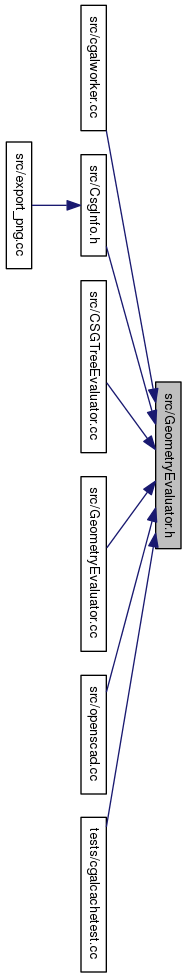
\includegraphics[height=1.37\columnwidth]{images/GeometryEvaluator_8h__dep__incl}
	\caption{Dependency graph of Geometery Evaluator}
	\label{fig:geometryevaluator8hdepincl}
\end{figure}

\begin{figure}[H]
	\centering
	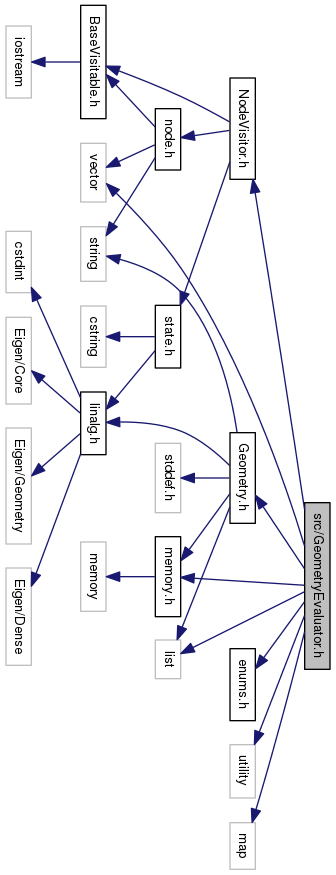
\includegraphics[height=1.37\columnwidth]{images/GeometryEvaluator_8h__incl}
	\caption{Caller graph of Geometery Evaluator}
	\label{fig:geometryevaluator8hincl}
\end{figure}

\begin{figure}[H]
	\centering
	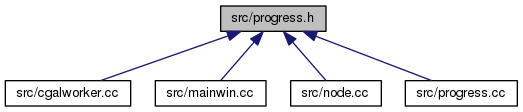
\includegraphics[width=\linewidth]{images/progress_8h__dep__incl}
	\caption{Caller graph of progress.h}
	\label{fig:progress8hdepincl}
\end{figure}

\begin{figure}
\centering
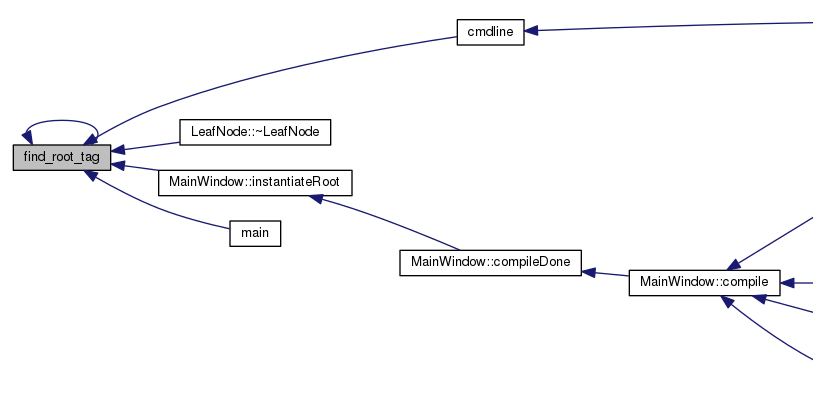
\includegraphics[width=\linewidth]{images/rootTag}
\caption{Caller Graph for find\_root\_tag}
\label{fig:findRootTag}
\end{figure}

\begin{figure}
\centering
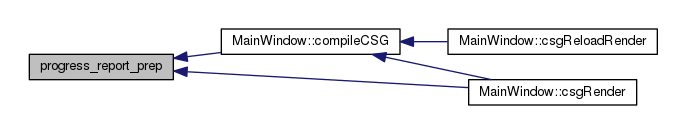
\includegraphics[width=\linewidth]{images/Prog}
\caption{Caller Graph for progress\_report\_prep}
\label{fig:prog}
\end{figure}
